% ******** Приклад оформлення документа за ДСТУ 3008-95 ********
% ******************** автор: Тавров Д. Ю. *********************

% зазначаємо стильовий файл, який будемо використовувати
\documentclass{udstu}

\addbibresource{refs.bib}

% починаємо верстку документа
\begin{document}

% створимо титульний аркуш
% за допомогою спеціальної команди
% \maketitlepage{params},
% де params --- це розділені комами пари "параметр={значення}"
\makediplomatitle{
% StudentName --- прізвище, ініціали студента
	StudentName={Скорденко Д. О.},
% StudentMale --- стать студента (true, якщо чоловік, false --- якщо жінка)
	StudentMale=true,
% StudentGroup --- група студента
	StudentGroup={КМ-01},
% Title --- назва
	Title={
		{\large Дипломна робота} \\
		на здобуття степеня бакалавра \\
		за освітньо-професійною програмою \invcommas{Наука про дані та математичне моделювання} \\
		спеціальності 113 \invcommas{Прикладна математика} \\
		на тему: \invcommas{Автоматичне маркування зображень за допомогою нейронних мереж}
	},
	Department={ПМА},
	HeadOfDepartment={Чертов Олег Романович},
% SupervisorDegree --- науковий ступінь, учене звання керівника роботи
% якщо наукового ступеня немає, можна відповідний рядочок пропустити
	SupervisorDegree={доцент кафедри ПМА},
% SupervisorName --- прізвище, ініціали керівника роботи
	SupervisorName={Сирота С. В.},
	ConsultDegree={доцент кафедри ПМА},
	ConsultName={Мальчиков В. В.}
}

% Створюємо анотацію
\abstractUkr

В даній роботі описано систему маркування зображень, в якій зроблено акцент на чотирьох апспектах:
висока точність, використання додаткової модальності, явна підсистема для передбачення к-сті лейблів, простота компонентів системи.

\paragraph{\textbf{Акутальність теми:}}
Все частіше виникає задача маркування зображення. Деякі із цих задач:
аналіз рентгенівських знімків, супутникових знімків, звичайних фотографій.
Для досягнення високої точності важливо аналізувати всі можливі аспекти даних
які надходять разом із задачею. Так для рентгенівських знімків - це може бути історія хвороб пацієнта,
для супутникових знімків - різні метадані, геолокація тощо, а для аналізу звичайних фотографій
- теги, анотації, метадані, тощо.
Відносно новим застосуванням даної моделі може бути структуризація зображень, згенерованих ШІ,
наприклад Stable Diffusion, де згенероване зображення - це основна модальність даних, а запит для його
генерування (prompt) - це додаткова.
Дана робота розглядає модульну систему, яку досить таки легко
адаптувати під кожну із наведених вище задач та досягнути високої точності.

\paragraph{\textbf{Мета дослідження:}}
Метою даної роботи є розробка ПЗ для маркування зображень (шпалерів робочого столу)
для покращення системи категоріального пошуку зображень (шпалерів робочого столу).

\paragraph{\textbf{Завдання дослідження:}}
Створити систему, яка буде виконувати маркування шпалерів на основі двох типів даних:
зображення та шумні теги, які опціонально надаються користувачами при завантаженні зображення на хостинг.

Також необхідно розв'язати наступні задачі:

\begin{itemize}
	\item Провести аналіз існуючих рішень
	\item Змоделювати систему
	\item Провести тренування системи
	\item Провести аналіз ефективності компонентів системи
	\item Порівнянти якость і повноту опису розглянутої моделі відносно існуючих рішень на основі тестових метрик
	\item Навести ілюстративні приклади роботи системи
\end{itemize}


\paragraph{\textbf{Об'єкт дослідження:}}
Об'єктом дослідження є маркування зображень, та методи покращення маркування зображення.
Для порівняння ефективності маркування серед існуючих рішень було обрано моделі,
для яких обраховані тестові метрики для того ж датасету, який обрано в даній роботі.
До множини існуючих рішень належать: SR-CNN-RNN \cite{sr-cnn-rnn}, Resnet-SRN \cite{srn},
MS-CMA \cite{cma}, Query2Label \cite{q2l}, Resnet-CPSD \cite{cpsd} та ін.

\paragraph{\textbf{Предмет дослідження:}}
Предметом дослідження є множина шпалерів робочого столу в якості основної модальності даних,
та додаткова інформація (надані людьми шумні теги) в якості додаткової.

\paragraph{\textbf{Кінцевий результат:}}
Кінцевим результатом даної роботи є математичне та програмне забезпечення, архітектура моделі,
вагові коефіцієнти натренованої моделі та код програмного забезпечення, в якому реалізовано дану роботу.


\shortings

\begin{itemize}[*]
	\item Модель - нейронна мережа
	\item Система (система для маркування зображень) - композиція моделей
	\item Задача класифікації - це задача, яка вирішує проблему приналежності чогось
	виключно до одного класу із довільного набору класів.
	\item Задача маркування - це задача, яка вирішує проблему приналежності чогось
	до декількох класів із довільного набору класів.
	\item DNN - Глибинна нейронна мережа (Deep Neural Network)
	\item CNN - Згорткова нейронна мережа (Convolutional Neural Network)
	\item RNN - Рекурсивна нейронна мережа (Recursive Neural Network)
	\item Тег (Tag) - шумна інформація надана користувачем у формі тексту
	(наприклад для зображення кота "Cat, Canada, Cola")
	\item Лейбл (Label) - синонім слова ground truth для класифікації
\end{itemize}


% створюємо зміст
\tableofcontents


% створюємо перший розділ роботи
\chapter{Вступ}

Задача класифікації - це одна із основних задач в аналізі зображень, вона полягає
у присвоєнні кожному зображенню один із класів. Таким чином дане формулювання накладає
обмеження - зображення містить тільки один об'єкт. Поява DNN \cite{dnn-cls}
та її подальший розвитком у CNN \cite{cnn-cls-1,cnn-cls-2} разом із створенням
великих датасетів як-от ImageNet \cite{deng2009imagenet} дало змогу вирішувати задачу
класифікації зображень значно швидше і якісніше ніж люди.

Зрозуміло, що зображення - це той тип даних, який у абсолютній більшості випадків містить більше одного об'єкта,
і відповідно більше одного класу для класифікації.
Для поглиблення опису існує задача маркування зображень (image labeling).
На відміну від класифікації, вона полягає у маркуванні зображення більше ніж одним класом.
Таким чином повнота опису зображення кратно зростає у порівннянні із звичайною класифікацією,
однак привносить декілька складних завдань.

По-перше, наявність декількох класів у одного зображення створює можливість
описувати значно ширший спектр візуальної інформації: різні об'єкти, стилі, дії, і тд.
Це створює потребу у розгляді додаткових джерел інформації, так як одного лиш зображення вже недостатньо.
Поява великих хостингів зображень таких як Imgur, Flickr, та ін., де користувачі можуть
як завантажувати різноманітні зображення, так і додавати до них описову інформацію у вигляді
тегів / анотацій, дала змогу створити досить різноманітні датасети: ImageNet \cite{deng2009imagenet},
MS-COCO \cite{cocodataset}, NUS-WIDE \cite{nus-wide-civr09}, та ін. Також існують і інші види датасетів,
наприклад: рентгенівські знімки та додаткова інформація (інші аналізи пацієнта, історія хвороб ...),
супутникові знімки та додаткова інформація у вигляді метаданих, геолокацій тощо.
Таким чином задача якісного маркування зображення вже охоплює значно більший спектр даних ніж просто
зображення.

По-друге, маркування зображень передбачає динамічну к-сть промаркованих класів,
так для опису зображенням із широким спектром понять необхідно 5-6 класів,
для зображення із простим вмістом - 2-3 класи.

По-третє, маркування зображень потребує оцінки якості проведеного маркування. Оскільки будь який
датасет буде містити в собі дизбаланс класів в тій чи іншій мірі, важливо оцінювати маркування із
урахуванням цього.

По-четверте, маркування зображень значно складніша задача ніж класифікація і відповідно зростає
складність моделей. З однієї сторони складніша модель потенційно здатна покращити якість маркування,
з іншої - може сильно збільшити як час на виконання маркування, так і час затрачений на тренування системи.
До складних систем належать ті, які використовують трансформери та/або мають велику к-сть параметрів.
Отже, важливо обрати певний баланс відносно складності моделі.

Все це робить задачу маркування зображення досить складною.


\chapter{Огляд існуючих рішень}

Розглянемо ключові аспекти задачі маркування зображення.

\paragraph{\textbf{Базове рішення}\\}

Базовим рішенням в задачі маркування зображення є аналіз основної модальності даних - зображення.
У абсолютній більшості існуючих робіт використовується CNN (Convolutional Neural Network).
Застосовуються різні архітекури даної моделі ResNet \cite{resnet}, AlexNet \cite{alexnet},
GoogleNet \cite{googlenet}, ResNext \cite{resnext}.
Спільним між ним є те що вони вже натреновані на великому датасеті, здебільшого ImageNet \cite{deng2009imagenet}.
Для адаптації моделі до обраного контексту така модель дотреновуєтсья (fine tune), замінюючи існуючий класифікатор
на класифікатор із адаптованою к-стю вихідних класів \cite{cnn-labeling}.
Це працює завдяки тому, що всі архітектури сучасних CNN моделей є багатошаровими,
і перші шари розпізнають базові особливості (features) зображення, а
останні шари вивчають більш глибинні особливості зображення,
таким чином дозволяючи адаптовувати модель під різні задачі після проведення підгонки (finetune).

\paragraph{\textbf{Додаткова модальність даних}\\}

Більш нові роботи також розглядають додаткові джерела інформації для підвищення якості та повноти
маркування зображень. Існує два основних підходи:

\begin{enumerate}
	\item \textit{Аналіз додаткової інформації.}
	Даний підхід аналізує додаткову до зображення інформацію.
	Це може бути як текстова інформація (теги / анотації) \cite{cnn-sinn,sr-cnn-rnn},
	так і метадані зображення \cite{cnn-neighbors,cnn-location}.
	Очевидним недоліком даного методу є потреба у цій додатковій інформації,
	яку можуть мати не всі зображення, а відсутність даної інформації
	знижує точність результуючого маркування.

	\item \textit{Аналіз цільових класів.}
	На відміну від загальної інтерпретації класів для задачі маркування
	(коли кожен клас - це незалежна сутність), даний підхід аналізує зв'язки між цільовими класами,
	створючи нову модальність на основі набору цільових класів \cite{srn}.
	Більш новим та узагальненим підходом є технологія word2vec (або аналогічне рішення), яка дозволяє,
	проаналізувавши набір слів, впорядкувати його у векторному просторі за семантичним значенням
	і побудувати граф, в якому вказуються класи (поняття) які часто знаходяться на одному зображенні
	(co-ocurrence; наприклад: риба, вода) та класи які рідко знаходяться
	на одному зображенні (dis-ocurrence; наприклад: риба, пустеля) \cite{q2l, cpsd, cma}.
	Перевагою даного підходу є те, що йому не потрібні ніякі нові дані крім зображень та
	відповідних їм цільових класів, а нова модальність, яка репрезентує зв'язок між класами
	створюється під час тренування системи. Основним недоліком таких систем полягає у
	високій складності, і як наслідок - довше по часу тренування / розпізнавання.
\end{enumerate}

\paragraph{\textbf{К-сть лейблів}\\}

Результатом роботи класифікаційної моделі є вектор ймовірностей, який репрезентує приналежність до класів.
Для задачі класифікації вибір результату на основі цього вектора очевидний - клас із найбільшою ймовірністю, однак
для задачі маркування все складніше.
Блільшість наведених вище робоіт розглядаєють задачу вибору к-сті лейблів як найкращі $k$ (top $k$) маркувань (\chaptername{ \ref{metrics}}),
де $k$ - наперед задана константа. Очевидно, що такий вибір к-сті класів не є оптимальним,
так як більш змістовні зображення будуть містити менше описової інформації і навпапки - менш змістовні будуть
містити лишню інформацію, яка до того ж може не мати нічого спільного із цим зображенням (\figurename{ \ref{figure:test-topk}})

\begin{figure}[!ht]
	\centering
	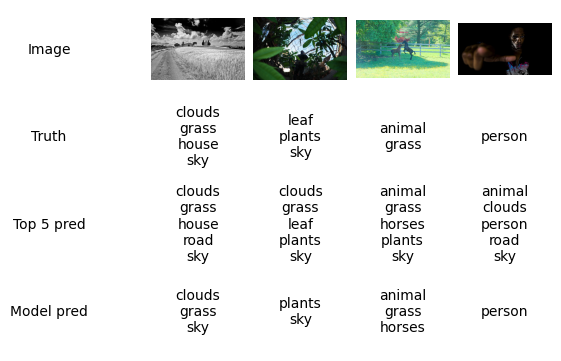
\includegraphics[width=0.9\textwidth]{PNG/test-topk-144}
	\caption{
	Приклад адаптивної к-сті лейблів.
	'Truth' - правдиве маркування,
	'Top 5 pred' - ілюстрація вибору top $k$, при $k=5$,
	'Model pred' - приклад роботи моделі
	}
	\label{figure:test-topk}
\end{figure}

Один із підходів як-от CNN-RNN \cite{cnn-rnn},
використовує RNN для аналізу візуальних даних (visual features) та автоматично виконує як задачу маркування,
так і задачу динамічного вибору кількості лейблів, однак в силу особливості RNN є певні обмеження
накладенні на порядок кодування класів.

Найновіші моделі \cite{q2l, cpsd, cma}, які розглядають зв'язок між цільовими класами, обирають
к-сть цільових класів на основі порогового значення (\chaptername{ \ref{metrics}}). Варто зазначити, що
даний підхід є ефективним тільки для цього типу моделей, так як вектор ймовірностей, який отримується на виході
даної моделі досить сильно дискретизований,
тобто для позитивного лейблу, який маркуєтсья 1 ймовірність буде $\approx 0.7-0.9$,
а для негативного, тобто 0 ймовірність $\approx 0.1-0.3$.


\chapter{Моделювання}

На основі проведного аналізу альтернатив, дана робота пропонує розглянути
модель, яка розглядає дві модальності даних: зображення та текстові теги.
Архітектура даного рішення складається із чотирьох компонентів (\figurename{ \ref{figure:composite}}).

\begin{figure}[!ht]
	\centering
	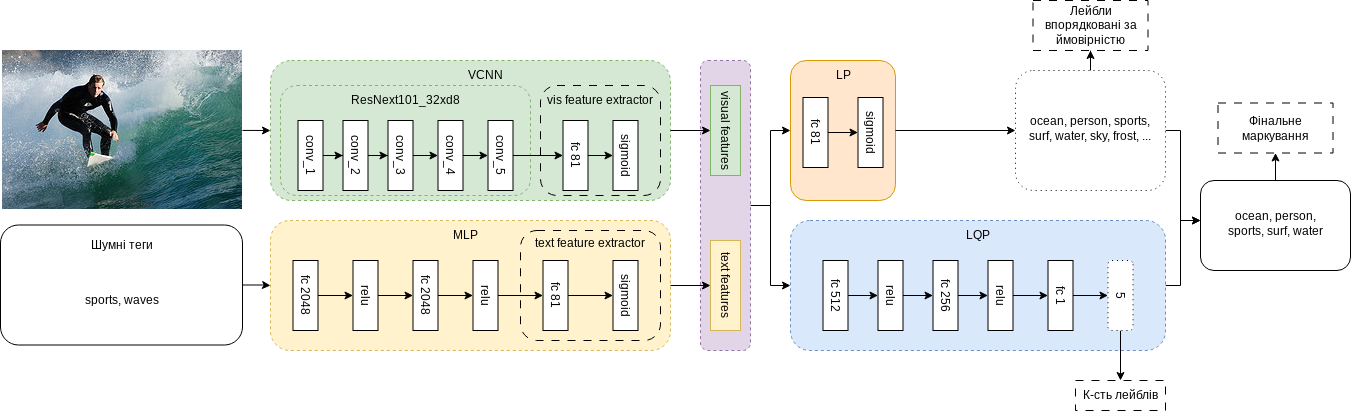
\includegraphics[width=1.0\textwidth]{PNG/composite}
	\caption{Архітектура композитної системи}
	\label{figure:composite}
\end{figure}


\section{VCNN}

Модель VCNN (\figurename{ \ref{figure:composite}}) призначена для вивчення особливостей (features) із зображення.
Отримує на вхід піселі зображення $I$, у формі матриці розмірності $(B,C,W,H)$, де
$B$ - к-сть зображень у групі для тегування,
$C$ - к-сть каналів у зображеннях зазвичай 1 або 3, Grey або RGB відповідно,
$W,H$ - розмірність зображень.

За базове рішення використовуєтсья ResNext101\_32x8d \cite{resnext} (сучасна версія resnet),
із адаптованим класифікатором (vis feature extractor), натреновану на датасеті ImageNet \cite{deng2009imagenet}.

На виході даної моделі ми отримуємо вектор вірогідностей $vf$ (visual feature vector),
який вказує вірогідність маркування зображення класом $j$ на основі візуальної інформації.


\section{MLP}

MLP (\figurename{ \ref{figure:composite}}) - аналізує текстові особливості (text features) тегів до зображення.
Теги до зображення $i$ репрезентуються як бінарний вектор $I = [1,0,1,0, ..., N]$,
де 1 - це наявність тегу, а $N$ - к-сть тегів.

Головна причина вибору звичайної MLP моделі для аналізу текстової інформації - це
те, що вхідна інформація - це шумні теги (наприклад: для фото кота - теги "Канада", "Кіт").

На виході даної моделі ми отримуємо вектор $tf$ вірогідностей (text feature vector),
який вказує вірогідність маркування зображення класом $j$ на основі текстової інформації.


\section{LP}

LP (\figurename{ \ref{figure:composite}}) - аналізує вектор вірогідності $v$,
який є композицією векторів $vf$ та $tf$: $v = [vf, tf]$.

На виході даної моделі ми отримуємо вектор вірогідностей, який комбінує інформацію отриману як із візуальної так і з
текстової інформації.


\section{LQP}

Модель LQP (\figurename{ \ref{figure:composite}}) аналізує кількість лейблів на основі вектору вірогідностей $v$,
який є композицією векторів $vf$ та $tf$: $v = [vf, tf]$.

Існує два підходи до визначення к-сті за допомогою нейронних мереж: класифікація та регресія.
LQP - регресійна модель.

Оскільки регресійні моделі досить швидко перенавчаються (overfitting), то необхідно задіяти регуляризацію.
В даній роботі, в якості регуляризатора задіяні Dropout шари \cite{dropout}, із вірогідністю відкидання (dropout rate) $0.5$.

На виході даної моделі є число, яке вказує на кількість лейблів у зображенні.


\section{Процес тренування}

Модель складається із декількох компонентів, що створює декілька проблемних місць під час тренування:
досить багато параметрів, дві різні цільові функції, проблема затухаючого градієнта, -
тому тренування відбуваєтсья у декілька стадій, у якому кожна із моделей тренується окремо
(деякі з них можна тренувати синхронно).


\paragraph{\textbf{Цільові функції}\\}

Для початку варто розглянути цільові функції (функція втрат, loss function).
Дані функції є базовим компонентом глибинного навчання.

В даній роботі використовуютсья дві функції: BCEWithLogitsLoss та MSELoss.

\paragraph{\textit{BCEWithLogitsLoss}\\}

Для тренування класифікаційних моделей (VCNN, MLP, LP) вихідні логіти $z_{ij}$
для групи (batch) зображень $I_N$ при $i = 1...N$, $j = 1...C$,
де $N$ - кількість зображень в групі, $C$ - кількість цільових класів,
цільова функція має вигляд:

\begin{equation}
\mathcal{L}_{cls} = \frac{1}{NC} \sum_{i}^{N} \sum_{j}^{C}
y_{ij} \cdot ln(\sigma(z_{ij})) + (1 - y_{ij}) \cdot ln(1 - \sigma(z_{ij}))
\end{equation}

, де $y_{ij} = 1$ якщо зображення $i$ анотоване класом $j$, інакше - $y_{ij} = 0$,
а $\sigma(\cdot)$ - це сигмоїдальна активаційна функція

\paragraph{\textit{MSELoss}\\}

Для тренування регресійної моделі LQP вихідні логіти $z_i$
для групи (batch) зображень $I_N$ при $i = 1...N$,
де $N$ - кількість зображень в групі,
цільова функція має вигляд:

\begin{equation}
\mathcal{L}_{reg} = \frac{1}{N} \sum_{i}^{N}
(y_i - z_i)^2
\end{equation}

, де $y_i$ - це кількість лейблів для зображення $I_i$.


\paragraph{\textbf{Тренування VCNN}\\}

Тренування моделі ResNext \cite{resnext} з нуля є досить складною задачою (дана модель має $\approx$ 80M параметрів),
адже для цього потрібні значні обчислювальні потужності.

Саме тому вироистовується натренована модель із адаптованим класифікатором (visual feature extractor) (\figurename{ \ref{figure:composite}}), яка підганяється (finetuned) на обраному датасеті.

Існує два підходи для підгонки:

\begin{enumerate}[1)]
	\item Підгонка всієї моделі:
	всі шари моделі підганяються (дотреновуються) з низькою швидкістю навчання (learning rate).
	Даний підхід вимагає великої обчислювальної потужності, однак надає високу точність та
	досить таки швидко тренується (в порівнянні із тренуванням з нуля).

	\item Підгонка класифікатора:
	відбуваєтсья тренування тільки класифікатора, фіксуючи всі інші параметри моделі.
	Даний підхід значно пришвидшує тренування в обмін на певну деградацію точності в порівнянні із 1-им варіантом.
\end{enumerate}

В даній роботі використовується 1 варіант підгонки, так як він надає вищу точність.


\paragraph{\textbf{Тренування MLP}\\}

Дана модель є звичайним багатошаровим персептроном, тому її тренування досить таки прямолінійне.


\paragraph{\textbf{Тренування LP}\\}

Дана модель призначена для обрахування вірогідностей на основі вектору $f = [vf, tf]$, оскільки вона
складається із одного шару то її тренування також очевидне.


\paragraph{\textbf{Тренування LQP}\\}

Дана модель є регресійною, її тренування також є очевидним, однак варто нормалізувати
вхідну к-сть лейблів, так як це пришвдшить та/або покращить збіжність моделі.


\section{Процес тестування}

\paragraph{\textbf{Тестування класифікаційних моделей (VCNN, MLP, LP)}\\}

Кожна із даних моделей обраховує вектор ймовірностей $P$,
для тестування необхідно перевести вектор ймовірностей (наприклад: $P = [0.9, 0.6, 0.1, 0.4, 0.6]$)
у вигляд маркування (наприклад: $M = [1,1,0,0,1]$). Дане перетворення називаєтсья індикаторною функцією.

\paragraph{Розглянемо два основних види індикаторної функції:}

\begin{enumerate}[1)]
	\item Порогове значення (threshold):
	для вектору ймовірностей $P$ та порогу $\alpha$ - вектор маркувань обраховується наступним чином:
	якщо $y_i > \alpha$, то маркуємо $1$, інакше $0$.
	Наприклад при $\alpha = 0.5$: $[0.9, 0.6, 0.1, 0.4, 0.6] \to [1,1,0,0,1]$.

	\item Найкращі $k$ (top $k$):
	для вектору ймовірностей $P$ та числа $k$ - вектор маркувань обраховується наступним чином:
	маркуємо $1$ найкращі $k$ ймовірностей, інакше $0$.
	Наприклад при $k = 4$: $[0.9, 0.6, 0.1, 0.4, 0.6] \to [1,1,0,1,1]$.
\end{enumerate}

Оскільки дані моделі \textbf{не передбачають} передбачення кількості лейблів,
то для тренування даних моделей використовується метод top $k$, при чому
$k = 3$.

\label{dynk}

Тобто для зображення $I$,
із маркуванням $Y = [1,0,0,0,1]$,
і вектором ймовірностей $P = [0.8,0.9,0.1,0.5,0.2]$
та результуючим вектором маркувань $M$:
$k = 3$, перетворення $P \to M \equiv [0.8,0.9,0.1,0.3,0.2] \to [1,1,0,1,0]$


\paragraph{\textbf{Тестування композитної моделі}\\}

Для тестування композитної моделі (\figurename{ \ref{figure:composite}})
необхідно обрахувати результуючі значення для моделей LP та LQP, і обрати
top $k$ лейблів LP, де $k$ - це передбачення LQP.


\chapter{Експерименти}

\section{Датасет}

Один із найбільш часто використовуваних датасетів для тестування моделей маркування зображень - NUS-WIDE \cite{nus-wide-civr09},
він складаєтсья із 269,655 зображень, 81 лейблу, та $\approx$ 5000 тегів в якості сторонньої текстової інформації.
Для проведення тренування/тестування використовується розподіл, надведений разом із
датасетом, так як він є збалансовний настільки, наскільки це можливо (\figurename{ \ref{figure:nus-wide-dist}}).

\begin{figure}[!ht]
	\centering
	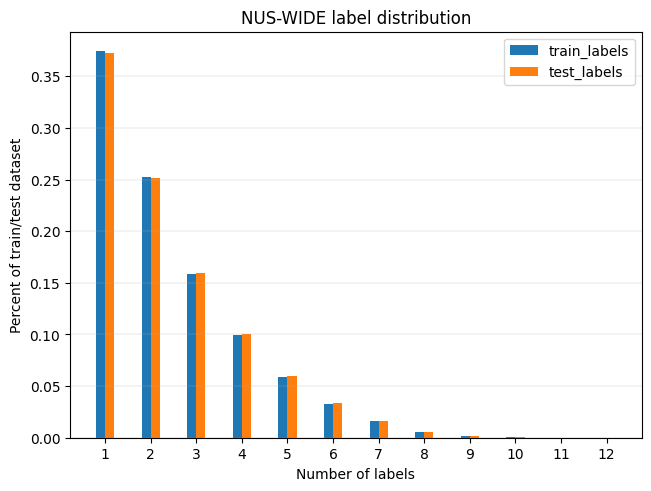
\includegraphics[width=0.9\textwidth]{PNG/nus-wide-dist}
	\caption{Розподіл лейблів у тренувальному/тестовому датасеті}
	\label{figure:nus-wide-dist}
\end{figure}

Важливо відмітити, що даний датасет містить посиланя на зображення на ресурсі Flickr, і деякої частина цих
зображень вже там немає. Також буде використано тільки 1000 найбільш частих тегів з $\approx$ 5000,
при чому зображення, які не містять жодного тега відфільтровано.

Далі наведено деякі числові характеристики тренувальної/тестової вибірок:

\begin{center}
\begin{tabular}{ccc}
		\toprule[2pt]
           & Тренування & Тестування \\
        \midrule
        Кількість зобаржень & 121962  & 81636 \\
        Середня к-сть лейблів & 2.42  & 2.43 \\
        Медіана к-сть лейблів & 2  & 2 \\
        Мінімальна к-сть лейблів & 1  & 1 \\
        Максимальна к-сть лейблів & 12  & 13 \\
        \bottomrule[2pt]
\end{tabular}
\captionof{table}{Характеристики тренувальної/тестової вибірок}
\end{center}

\clearpage


\section{Метрики}
\label{metrics}

Для оцінки точності будуть використовуватись метрики, які є загально вживаними для оцінки
задачі маркування зображень (multi-label image annotation).

\begin{equation}
\begin{aligned}
\textnormal{С-P} &= \frac{1}{C} \sum_{j=1}^C \frac{NI^c_j}{NI^p_j} & \textnormal{O-P} &= \frac{\Sigma^N_{i=1} NL^c_i}{\Sigma^N_{i=1} NL^p_i} \\
\textnormal{C-R} &= \frac{1}{C} \sum_{j=1}^C \frac{NI^c_j}{NI^g_j} & \textnormal{O-R} &= \frac{\Sigma^N_{i=1} NL^c_i}{\Sigma^N_{i=1} NL^g_i} \\
\textnormal{C-F1} &= \frac{2 \cdot \textnormal{C-P} \cdot \textnormal{C-R}}{\textnormal{C-P} + \textnormal{C-R}} & \textnormal{O-F1} &= \frac{2 \cdot \textnormal{O-P} \cdot \textnormal{O-R}}{\textnormal{O-P} + \textnormal{O-R}} \\
\end{aligned}
\end{equation}

,де \begin{itemize}[*]
        \item $C$ - к-сть класів
        \item $N$ - к-сть тестових зображень
        \item $NI^c_j$ - к-сть зображень які \textbf{коректно} промарковано як клас $j$
        \item $NI^g_j$ - к-сть зображень які мають клас $j$
        \item $NI^p_j$ - к-сть зображень які промарковано як клас $j$
        \item $NL^c_i$ - к-сть \textbf{коректно} промаркованих лейблів для зображення $i$
        \item $NL^g_i$ - к-сть лейблів які має зображення $i$
        \item $NL^p_i$ - к-сть промаркованих лейблів для зображення $i$
\end{itemize}

Варто відзначити, що дані метрики є зміщеними (biased),
при чому по-класові метрики (C) зміщені в сторону рідкісних класів,
а загальні метрики (O) - в сторону частих класів \cite{cnn-labeling}.

\clearpage

Для того щоб отримати унфіормене представлення про ефективність моделі
буде використовуватись наступна метрика,
яка бере до уваги як C-F1 так і O-F1, що полегшує інтерпретацію результатів:

\begin{equation}
\text{H-F1} = \frac{2 \cdot \text{C-F1} \cdot \text{O-F1}}{\text{C-F1} + \text{O-F1}}
\end{equation}


\clearpage


\section{Тренування}

Для програмної реалізації запропонованої моделі було використано PyTorch.

Оскільки в даній роботі, використовується модель ResNext \cite{resnext} натренована
на датасеті ImageNet \cite{deng2009imagenet}, то для вхідних зображень потрібно
застосувати певне перетворення:

\begin{enumerate}[1)]
	\item Зміна розміру (Resize) $232 \times 232$,
	використовуючи білінійну інтерполяцію
	\item Центральний кроп (Central crop) $224 \times 224$
	\item Зміна масшатбу (Rescale) [0,1]
	\item Нормалізація на основі статистичних величин ImageNet \cite{deng2009imagenet}.
	А саме: mean = [0.485, 0.456, 0.406] та std = [0.229, 0.224, 0.225]
\end{enumerate}

Дане перетворення доступно у біблоітеці PyTorch.


\paragraph{\textbf{Параметри навчання}\\}

Класифікаційні моделі VCNN та MLP навчались із
швидкістю навання (learning rate) 0.001, а LP - зі швидкістю 0.01.
Також для начання цих трьох моделей використовувався контроллер швикдості навчання
(learning rate scheduler), який множив швидкість навчання на 0.5, досягаючи
5-ої та 10-ої епохи.

Регресійна модель LQP навчалась із сталою швидкістю навчання (learning rate) 0.0005.

Для всіх навчання всіх вище згаданих моделей використовувався оптимізатор
AdamW, із параметром l1 регуляризації (weight decay) 0.0003.

Розмір групи (batch size) 32.

Також варто відзначити, що в даній роботі епоха - це 20\% від усіх даних,
при чому після кожної епохи дані перемішуються (shuffle), отримаючи
нові 20\% даних.


\paragraph{\textbf{Процес навчання}\\}

Для тренування було використано графічний процесор 'Nvidia L4'.
Для тренування всіх елементів моделі знадобилось $\approx$ 3 години.

Для оптимізації процесу тренування було застосовано техніку mixed precision,
яка використовує f16 замість f32, під час певних етапів тренування \cite{mixed-precision}.


\begin{figure}[h]
\centering
	\subcaptionbox{Навчання VCNN}
		{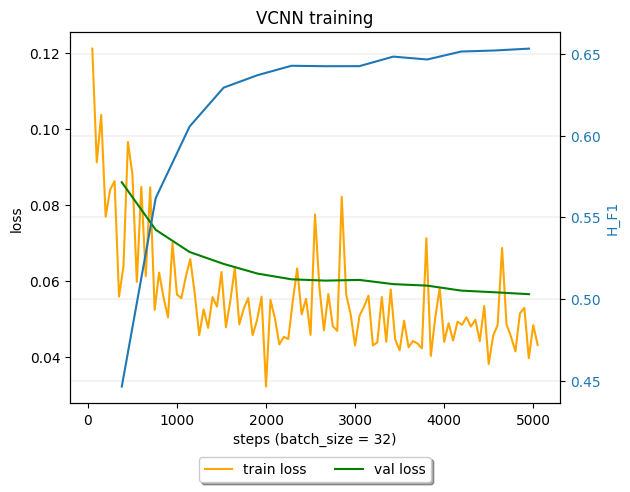
\includegraphics[width=0.45\linewidth]{PNG/vcnn-train}}
	\subcaptionbox{Навчання MLP}
		{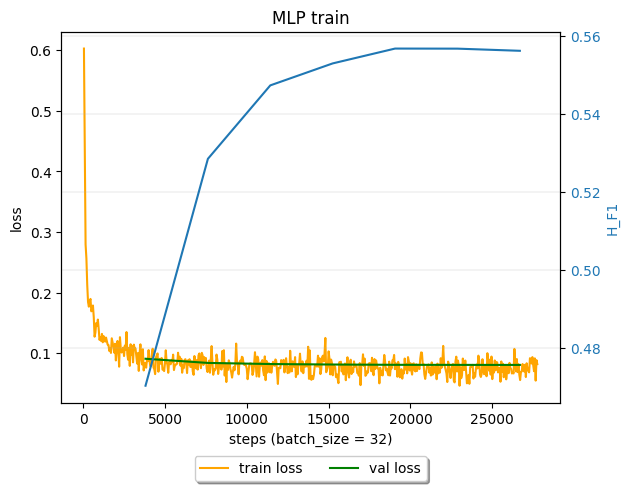
\includegraphics[width=0.45\linewidth]{PNG/mlp-train}}
	\subcaptionbox{Навчання LP}
		{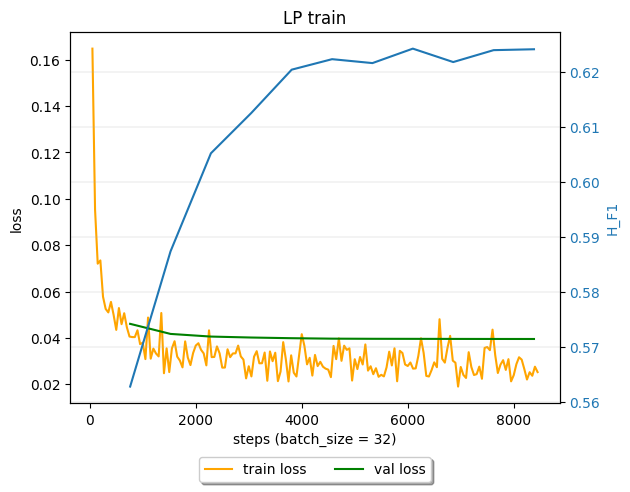
\includegraphics[width=0.45\linewidth]{PNG/lp-train}}
	\subcaptionbox{Навчання LQP}
		{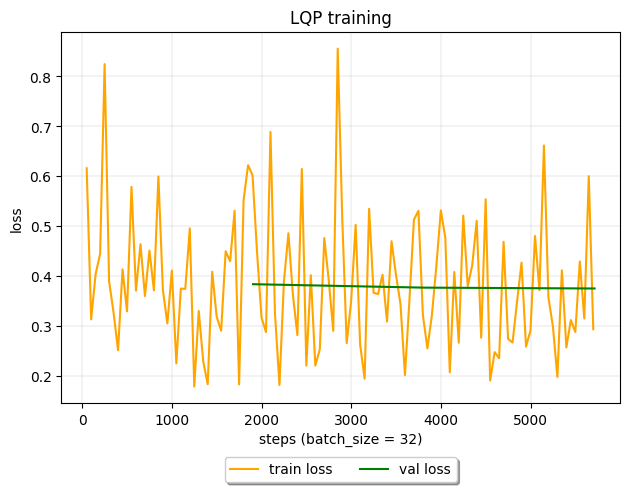
\includegraphics[width=0.45\linewidth]{PNG/lqp-train}}
\caption{Процес навчання моделей}
\end{figure}

\chapter{Аналіз результатів}

\section{Аналіз компонентів системи}

\begin{center}
\resizebox{\textwidth}{!}{\begin{tabular}{l|c|c|ccc|ccc|c}
		\toprule[2pt]
		Модель & Індикаторна ф-ція (\ref{dynk}) & Модальність & C-P & C-R & C-F1 & O-P & O-R & O-F1 & H-F1 \\
        \midrule
        Композитна  & top k & Зображення+теги & 72.49 & 59.51 & 65.36 & 76.53 & 74.41 & 75.46 & 70.04 \\
        VCNN+MLP+LP & top 3 & Зображення+теги & 60.51 & 61.28 & 60.89 & 67.87 & 71.52 & 63.98 & 62.40 \\
        VCNN+LQP    & top k & Зображення  & 64.62 & 37.61 & 47.54 & 77.07 & 59.01 & 66.84 & 55.56 \\
		VCNN        & top 3 & Зображення  & 44.48 & 53.32 & 48.50 & 55.44 & 68.52 & 61.29 & 54.15 \\
        \bottomrule[2pt]
\end{tabular}}
\captionof{table}{Порівняння компонентів моделі}
\end{center}

Результуюча композитна модель показала значно кращий результат ніж базове рішення (VCNN).

\paragraph{\textbf{Додаткова модальність (MLP+LP)}\\}

Додавання додаткової модальності у вигляді тегів внесло значний вклад
у підвищення якості маркування.
Порівнюючи відповідні метрики H-F1 для моделей VCNN та VCNN+MLP+LP, можна
побачити приріст на $8.25\%$. При чому варто відзначити, що цей ріст в основному
забезпечений приростом метрики C-F1, яка є зміщеною в сторону більш рідкісних класів.
Варто відзначити, що це працює завдяки тому що зазвичай теги надані користувачами відмічають
досить рідкісні поняття, які на відміну від частих тегів (небо, сонце, людина, вода і тд.) складно
розпізнати маючи одне лиш зображення.

\paragraph{\textbf{Передбачення кількості лейблів (LQP)}\\}

При використанні компоненту LQP кількість лейблів обирається за принципом 'top k', а не 'top 3' (\ref{dynk}).
Це очевидним чином підвищує точність фінального  маркування, адже деякі зображення можуть мати більше трьох лейблів,
інші - менше трьох. Порівнюючи вплив компоненти LQP для базового рішення (VCNN) та композитної моделі (VCNN+MLP+LP+LQP)
можна зробити припущення, що VCNN аналізує загальні поняття на зображенні, а враховуючи дизбаланс класів у датасеті,
використання принципу 'top k' збільшує точність (precision), сильно жертвуючи по-класовим охопленням (C-R), і,
як наслідок, не сильно збільшуючи величину головної метрики H-F1. На практиці це виливалось у те, абсолютна більшість
зображень маркувалась частими лейблами (людина, вода, небо і тд.), а рідкісні теги - ігнорувались.
Натомість у композитній моделі вищезгаданий принцип чудово проявив себе.
Згідно із тестовими метриками покращення становить $7.64\%$.


\section{Порівнняня з існуючими рішеннями}

\begin{center}
\resizebox{\textwidth}{!}{\begin{tabular}{l|c|c|ccc|ccc|c}
	\toprule[2pt]
	Модель & Індикаторна ф-ція (\ref{dynk}) & Модальність & C-P & C-R & C-F1 & O-P & O-R & O-F1 & H-F1 \\
	\midrule
	Композитна  & top k & Зображення+теги & 72.49 & 59.51 & 65.36 & 76.53 & 74.41 & 75.56 & 70.04 \\
	\hline
	Query2Label \cite{q2l} & threshold $\alpha$ & Зображення (+аналіз класів) & - & - & 67.60 & - & - & 76.3 & 71.69 \\
	SR-CNN-RNN \cite{sr-cnn-rnn} & top 3 & Зображення+теги (+аналіз класів) & 71.73 & 61.73 & 66.36 & 77.41 & 76.88 & 77.15 & 71.35 \\
	Resnet-CPSD \cite{cpsd} & threshold $\alpha$ & Зображення (+аналіз класів) & - & - & 64.00 & - & - & 75.30 & 69.19 \\
	MS-CMA \cite{cma} & threshold $\alpha$ & Зображення (+аналіз класів) & - & - & 60.50 & - & - & 73.80 & 66.49 \\
	Resnet-SRN \cite{srn} & threshold 0.5 & Зображення (+аналіз класів) & 65.20 & 55.80 & 58.50 & 75.50 & 71.50 & 73.40 & 65.10 \\
	SINN \cite{cnn-sinn}  & top 3 & Зображення+теги & 58.30 & 60.63 & 59.44 & 57.05 & 79.12 & 66.29 & 62.68 \\
	TagNeighbour \cite{cnn-neighbors}  & top 3 & Зображення+метадані & 54.74 & 57.30 & 55.99 & 53.46 & 75.10 & 62.46 & 59.05 \\
	CNN+Logistic \cite{cnn-sinn}  & top 3 & Зображення  & 45.60 & 45.03 & 45.31 & 51.32 & 70.77 & 59.50 & 51.44 \\
	CNN-RNN \cite{cnn-rnn}  & top 3 & Зображення  & 40.50 & 30.40 & 34.70 & 49.9 & 61.70 & 55.20 & 42.61 \\
	CNN+WARP \cite{cnn-labeling}  & top 3 & Зображення  & 31.65 & 35.60 & 33.51 & 48.59 & 60.49 & 53.89 & 41.32 \\
	CNN+Softmax \cite{cnn-labeling}  & top 3 & Зображення  & 31.68 & 31.22 & 31.45 & 47.82 & 59.52 & 53.03 & 39.48 \\
	\bottomrule[2pt]
\end{tabular}}
\label{table:models-metrics}
\captionof{table}{Порівняння результуючих метрик для різних моделей на датасеті NUS-WIDE}
\end{center}


\paragraph{\textbf{Точність запропонованого рішення}}
Композитна модель (VCNN+MLP+LP+LQP) продемонструвала високу якість маркування на тестових метриках у порівнянні
із розглянутими альтернативними рішеннями. Згідно із метрикою H-F1 запропоноване рішення є третім.

\paragraph{\textbf{Модальність даних}}
Задача маркування зображень розглядає зображення як основну модальність, однак додавання модальності,
очікувано, покращує результати маркування. Це підтверджують метрики наведені в \tablename{ \ref{table:models-metrics}}.
Серед розглянутих рішень є 3 варіанти модальності даних з якимим працюють нейронні мережі.
Найменш ефективним, як і очікувалось, виявились моделі які аналізують виключно зображення.
Введення інших двох видів додаткових модальностей: теги, аналіз класів, - надають значно кращі результати.
Варто відзначити, - аналіз класів (найкраще імплементовано в: Query2Label \cite{q2l}, Resnet-CPSD
\cite{cpsd} та MS-CMA \cite{cma}) не потребує ніяких додактових даних окрім зображення,
що є вагомою конкурентною перевагою, враховуючи незначну відміність в точності моделей.

\paragraph{\textbf{Індикаторна функція}}
Для оцінки ефективності запропонованої індикаторної функції 'top k', варто ізолювати вплив саме цієї фнкції.
Для ціього розглянемо існуючі моделі, які працюють із тією ж модальністю даних. Найкращою із таких моделей є
SINN \cite{cnn-sinn}. Використання під-системи LQP, яка передбачає роботу із динамічною кількістю лейблів при маркуванні
(top k) значено підвищує якість. Згідно із наведеними метриками покращення складає
$7.36\%$ (\tablename{ \ref{table:models-metrics}}), що є вагомим приростом.


\clearpage

\section{Демонстративні приклади}

З тестового датасету випадковим чином обрано декілька зображень, для демонстрації роботи моделі:

\begin{figure}[h]
\centering
	\subcaptionbox{}
		{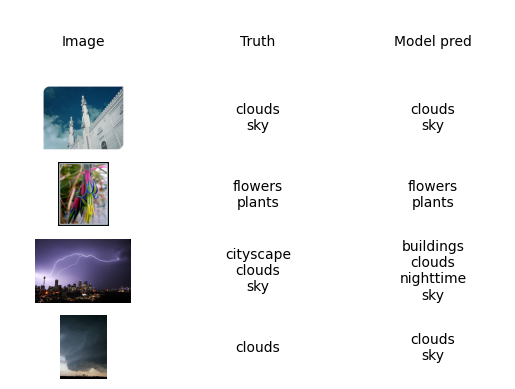
\includegraphics[width=0.45\linewidth]{PNG/showcase-1-20}}
		\label{figure:showcase-1}
	\subcaptionbox{}
		{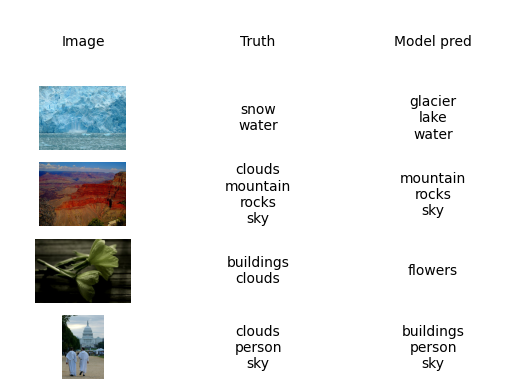
\includegraphics[width=0.45\linewidth]{PNG/showcase-2-30}}
		\label{figure:showcase-2}
	\subcaptionbox{}
		{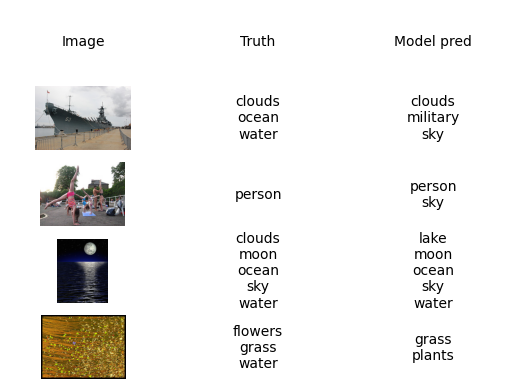
\includegraphics[width=0.45\linewidth]{PNG/showcase-3-40}}
 	\subcaptionbox{}
 		{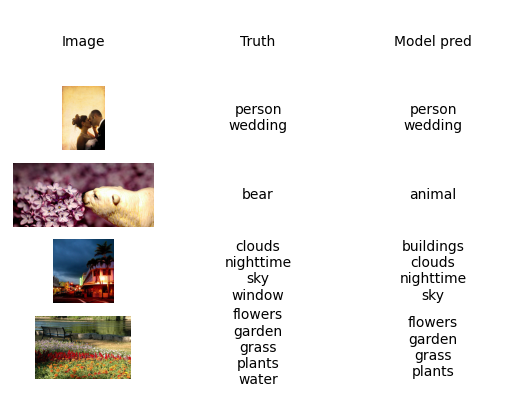
\includegraphics[width=0.45\linewidth]{PNG/showcase-4-70}}
\caption{Демонстративні приклади}
\end{figure}

Задамо умовне позначення "а::1", що означає демонстративний приклад "а", перше зображення зверху,
"в::2" - приклад "в", друге зображення зверху і тд.

Серед наведених прикладів можна розглянути кілька цікавих моментів, які не відображають тестові метрики:

\begin{itemize}[*]
	\item Іноді модель передбачає маркування, якого немає у датасеті, однак присутнє на зображені.
	Наприклад: [а::3,а::4,б::1,б::3,б::4,в::1,в::2,г::2,г::3].
	\item Існують випадки коли модель відмічає поняття, які не можуть бути присутніми на одному зображенні.
	Це є прямим наслідком того, що наша модель розглядає цільові класи як незалежі сутності.
	Наприклад: lake та ocean як-от в прикладі 'в::3'.
	\item Іноді передбачення моделі відсікають неіснуючі поняття та маркують зображення краще ніж це
	було зроблено в датасеті. Так для зображення 'б::3' на якому зображено якусь рослину датасет
	вказує що це: 'buildings, clouds'; а модель - 'flowers'.
\end{itemize}

Окрім наведених вище особливих випадків, іноді модель, звичайно, помиляється. Однак у наведених
прикладах немає значних помилок у маркуванні.

% створюємо Висновки
\conclusions

В даній роботі було розглянуто композитну модель, для маркування зображень (шпалерів робочого столу)
проведено оцінювання її точності на тестових метриках.

Розглянута модель показала хороший результат у порівнянні із існуючими альтернативними рішеннями.

\textit{До переваг розглянутого рішення належать:}

\begin{itemize}[+]
	\item Висока точність
	\item Невелика кількість параметрів ($\approx 95\%$ параметрів має модель для аналізу зображень)
	\item Висока швидкість тренування
\end{itemize}

\textit{Недоліками є:}

\begin{itemize}[-]
	\item Неможливість тренування моделі в один етап (end-to-end)
	\item Необхідність використання додаткових даних (тегів) для
	отримання високої якості опису зображення
\end{itemize}

В подальшому варто розглянути ефективність даної моделі на інших датасетах (наприклад MSCOCO \cite{cocodataset}).
також варто розглянути і методи для аналізу цільових класів, так як незважаючи на
значне ускладнення фінальної моделі це надає досить високий приріст до точності маркування.

Результуюча композитна модель збережена у форматі safetensors.

Після проведеного дослідження було висунуто гіпотезу, що дане рішення можна застосувати
і у інших схожих предметних областях. Так для аналізу рентгенівських знімків - це може бути історія хвороб пацієнта,
для супутникових знімків - різні метадані, геолокація тощо, а для аналізу звичайних фотографій
- теги, анотації, метадані, тощо.

\printbibliography

\append{Код лістинг}

Код міститься у github репозиторії \underline{\href{https://github.com/skorodenko/wallpaper\_tagging}{Посилання}}

Далі наведено загальний опис елементів проекту:


\paragraph{\textbf{Дані:}\\}

Файли в директорії scripts 'nuswide2ndjson.py' та '1ktags.py' призначенні для обробки
сирих даних із датасету в формат ndjson для подальшого тренування.

Файл data.py містить адаптери та визначення датасету для тренування.


\paragraph{\textbf{Тренування:}\\}

Скрипти для тренування для всіх моделей (VCNN, MLP, LP, LQP) знаходяться в директорії
'scripts/train'.


\paragraph{\textbf{Тестування:}\\}

Скрипт для тестування моделей: 'scripts/test.py'.
Даний скрипт передбачає тестування як фінальної моделі, так і деяких конфігурацій її компонентів.


\paragraph{\textbf{Інше:}\\}

Скрипт 'scripts/compose2safe.py' призначений для конвертації вагів моделей (VCNN, MLP, LP, LQP)
формату .ckpt у композитну модель формату .safetensors.

Ноутбук 'testing.ipynb' призначений для наглядного тестування моделі.


\append{Додаткові приклади}

\begin{figure}[!ht]
	\centering
	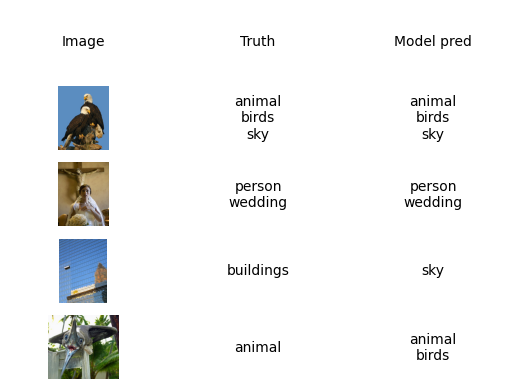
\includegraphics[width=0.9\textwidth]{PNG/showcase-100}
	\caption{}
\end{figure}

\begin{figure}[!ht]
	\centering
	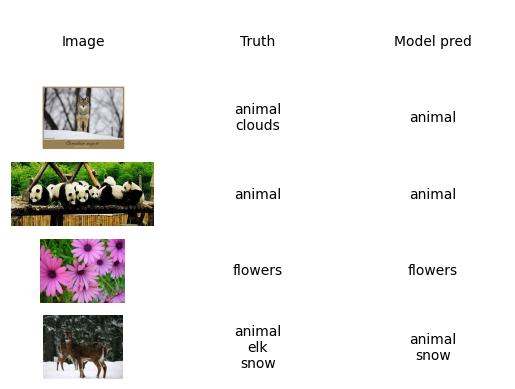
\includegraphics[width=0.9\textwidth]{PNG/showcase-125}
	\caption{}
\end{figure}

\begin{figure}[!ht]
	\centering
	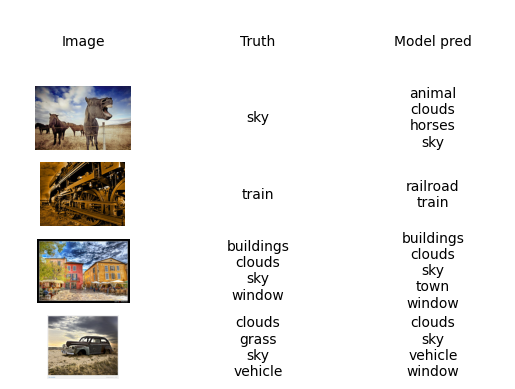
\includegraphics[width=0.9\textwidth]{PNG/showcase-150}
	\caption{}
\end{figure}

\begin{figure}[!ht]
	\centering
	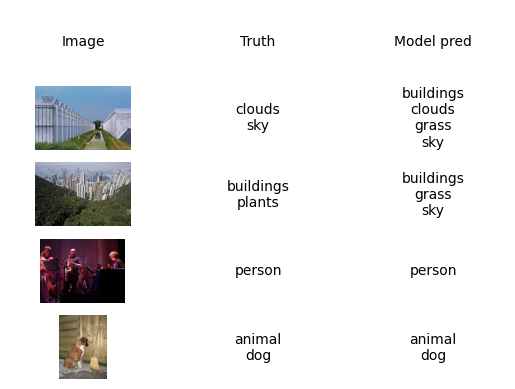
\includegraphics[width=0.9\textwidth]{PNG/showcase-175}
	\caption{}
\end{figure}

\begin{figure}[!ht]
	\centering
	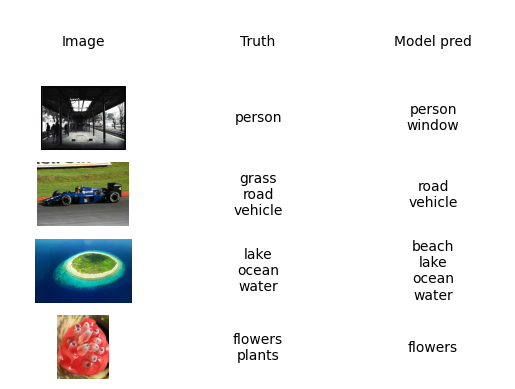
\includegraphics[width=0.9\textwidth]{PNG/showcase-200}
	\caption{}
\end{figure}

\begin{figure}[!ht]
	\centering
	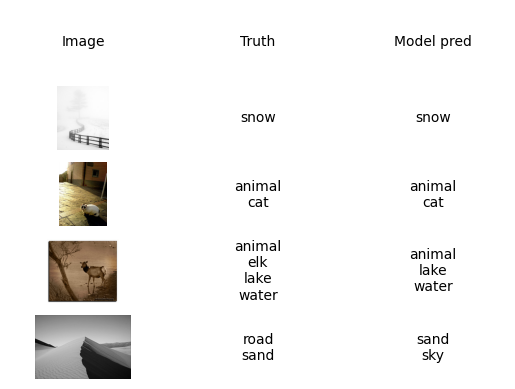
\includegraphics[width=0.9\textwidth]{PNG/showcase-225}
	\caption{}
\end{figure}

\begin{figure}[!ht]
	\centering
	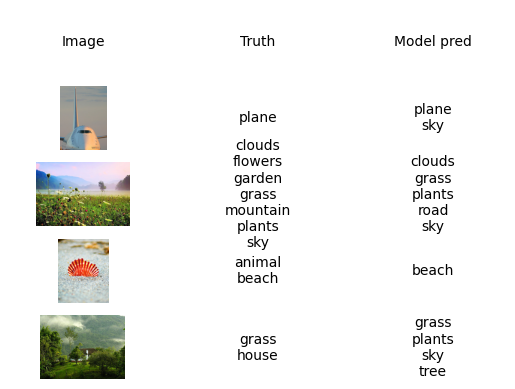
\includegraphics[width=0.9\textwidth]{PNG/showcase-250}
	\caption{}
\end{figure}

\begin{figure}[!ht]
	\centering
	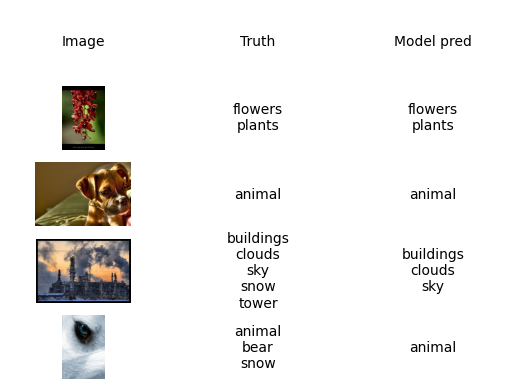
\includegraphics[width=0.9\textwidth]{PNG/showcase-275}
	\caption{}
\end{figure}

\begin{figure}[!ht]
	\centering
	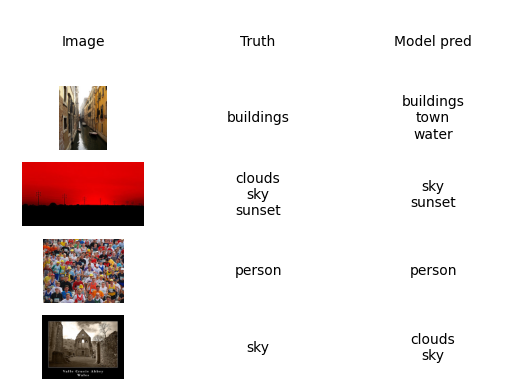
\includegraphics[width=0.9\textwidth]{PNG/showcase-300}
	\caption{}
\end{figure}

\begin{figure}[!ht]
	\centering
	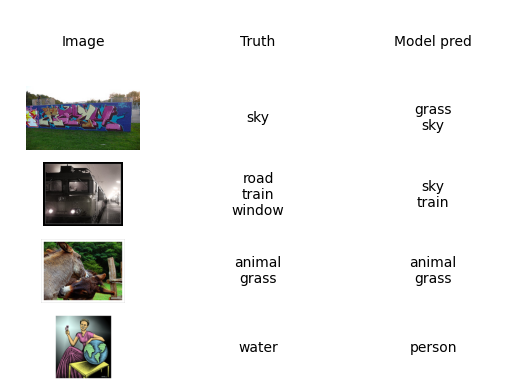
\includegraphics[width=0.9\textwidth]{PNG/showcase-325}
	\caption{}
\end{figure}

\begin{figure}[!ht]
	\centering
	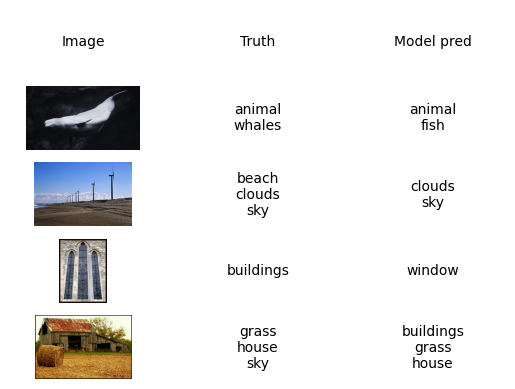
\includegraphics[width=0.9\textwidth]{PNG/showcase-350}
	\caption{}
\end{figure}

\begin{figure}[!ht]
	\centering
	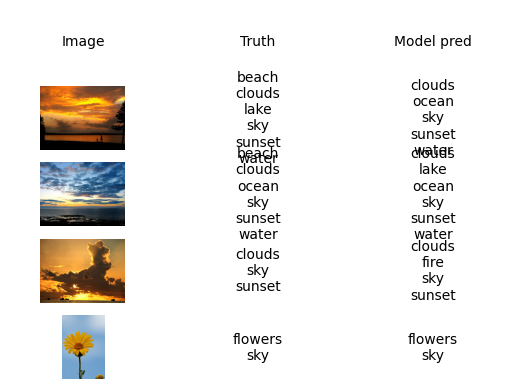
\includegraphics[width=0.9\textwidth]{PNG/showcase-375}
	\caption{}
\end{figure}

\begin{figure}[!ht]
	\centering
	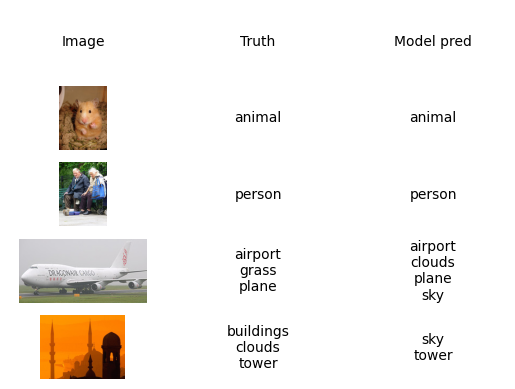
\includegraphics[width=0.9\textwidth]{PNG/showcase-400}
	\caption{}
\end{figure}

\end{document}
